\noindent
\begin{minipage}[t]{0.25\textwidth}
    \vspace*{0pt}
    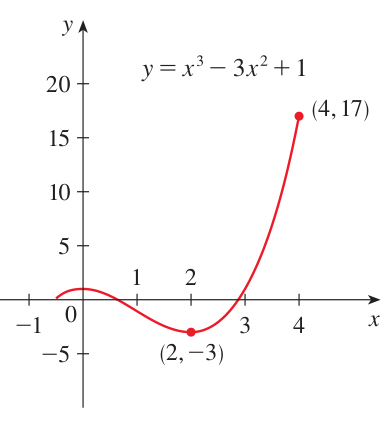
\includegraphics[width=\linewidth]{images/p0320_fig1.png}
    \par\vspace{3pt}
    \noindent{\small\textbf{\textsf{HÌNH 15}}}

    \vspace{18pt}
    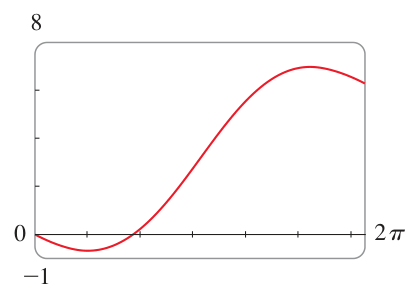
\includegraphics[width=\linewidth]{images/p0320_fig2.png}
    \par\vspace{3pt}
    \noindent{\small\textbf{\textsf{HÌNH 16}}}

    \vspace{38pt}
    \noindent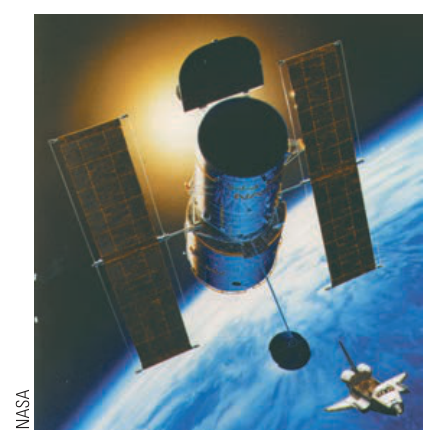
\includegraphics[width=\linewidth]{images/p0320_fig3.png}
\end{minipage}%
\hfill
\begin{minipage}[t]{0.72\textwidth}
    \vspace*{0pt}
    \noindent
    So sánh bốn giá trị này, ta thấy giá trị lớn nhất tuyệt đối là $f(4) = 17$ và giá trị nhỏ nhất tuyệt đối là $f(2) = -3$.

    Trong ví dụ này, giá trị lớn nhất tuyệt đối đạt được tại một điểm đầu mút, trong khi giá trị nhỏ nhất tuyệt đối đạt được tại một số tới hạn. Đồ thị của $f$ được phác họa trong Hình 15.\hfill{\color{stewartcyan}$\blacksquare$}

    \vspace{8pt}
    Nhờ phần mềm vẽ đồ thị hoặc máy tính bỏ túi có chức năng đồ họa, ta có thể ước lượng các giá trị lớn nhất và nhỏ nhất một cách rất dễ dàng. Nhưng, như ví dụ tiếp theo cho thấy, phép tính vi tích phân là cần thiết để tìm ra các giá trị \emph{chính xác}.

    \vspace{8pt}
    \noindent
    \textbf{\textsf{\color{stewartcyan}VÍ DỤ 9}}\enspace \textbf{\textsf{\color{stewartcyan}(a)}}\enspace Sử dụng máy tính cầm tay hoặc máy vi tính để ước lượng các giá trị nhỏ nhất và lớn nhất tuyệt đối của hàm số $f(x) = x - 2 \sin x$, $0 \le x \le 2\pi$.\par
    \noindent
    \textbf{\textsf{\color{stewartcyan}(b)}}\enspace Sử dụng phép tính vi tích phân để tìm các giá trị nhỏ nhất và lớn nhất chính xác.

    \vspace{6pt}
    \noindent
    \textbf{\textsf{\color{stewartcyan}LỜI GIẢI}}\enspace \textbf{\textsf{\color{stewartcyan}(a)}}\enspace Hình 16 thể hiện đồ thị của $f$ trong hình chữ nhật quan sát $[0, 2\pi] \times [-1, 8]$. Giá trị lớn nhất tuyệt đối vào khoảng $6{,}97$ và đạt được khi $x \approx 5{,}24$. Tương tự, giá trị nhỏ nhất tuyệt đối vào khoảng $-0{,}68$ và đạt được khi $x \approx 1{,}05$. Ta có thể thu được các ước lượng số chính xác hơn, nhưng để có các giá trị chính xác, chúng ta phải sử dụng phép tính vi tích phân.\par

    \vspace{4pt}
    \noindent
    \textbf{\textsf{\color{stewartcyan}(b)}}\enspace Hàm số $f(x) = x - 2 \sin x$ liên tục trên $[0, 2\pi]$. Vì $f'(x) = 1 - 2 \cos x$, ta có $f'(x) = 0$ khi $\cos x = \frac{1}{2}$ và điều này xảy ra khi $x = \pi/3$ hoặc $5\pi/3$. Các giá trị của $f$ tại các số tới hạn này là
    \begin{align*}
        f(\pi/3) &= \frac{\pi}{3} - 2 \sin \frac{\pi}{3} = \frac{\pi}{3} - \sqrt{3} \approx -0{,}684853 \\[3pt]
        \llap{\text{và}\qquad} f(5\pi/3) &= \frac{5\pi}{3} - 2 \sin \frac{5\pi}{3} = \frac{5\pi}{3} + \sqrt{3} \approx 6{,}968039
    \end{align*}
    Các giá trị của $f$ tại các điểm đầu mút là
    \[
        f(0) = 0 \qquad\qquad f(2\pi) = 2\pi \approx 6{,}28
    \]
    So sánh bốn giá trị này và sử dụng Phương pháp khoảng đóng, ta thấy giá trị nhỏ nhất tuyệt đối là $f(\pi/3) = \pi/3 - \sqrt{3}$ và giá trị lớn nhất tuyệt đối là $f(5\pi/3) = 5\pi/3 + \sqrt{3}$. Các giá trị từ phần (a) đóng vai trò kiểm tra lại kết quả tính toán của chúng ta.\hfill{\color{stewartcyan}$\blacksquare$}

    \vspace{8pt}
    \noindent
    \textbf{\textsf{\color{stewartcyan}VÍ DỤ 10}}\enspace Kính viễn vọng không gian Hubble được triển khai vào ngày 24 tháng 4 năm 1990 bởi tàu con thoi \emph{Discovery}. Một mô hình cho vận tốc của tàu con thoi trong sứ mệnh này, từ khi cất cánh tại $t = 0$ cho đến khi các tên lửa đẩy nhiên liệu rắn được tách rời tại $t = 126$ giây, được cho bởi
    \[
        v(t) = 0{,}001302t^3 - 0{,}09029t^2 + 23{,}61t - 3{,}083
    \]
    (tính bằng feet trên giây). Sử dụng mô hình này, hãy ước lượng các giá trị lớn nhất và nhỏ nhất tuyệt đối của \emph{gia tốc} tàu con thoi trong khoảng thời gian từ khi rời bệ phóng đến khi tách các tên lửa đẩy.\par

    \vspace{6pt}
    \noindent
    \textbf{\textsf{\color{stewartcyan}LỜI GIẢI}}\enspace Chúng ta được yêu cầu tìm các giá trị cực trị không phải của hàm vận tốc đã cho, mà là của hàm gia tốc. Vì vậy, trước tiên ta cần lấy đạo hàm để tìm gia tốc:
    \begin{align*}
        a(t) = v'(t) &= \frac{d}{dt}\left(0{,}001302t^3 - 0{,}09029t^2 + 23{,}61t - 3{,}083\right) \\[3pt]
        &= 0{,}003906t^2 - 0{,}18058t + 23{,}61
    \end{align*}
\end{minipage}
